\chapter{Maximizing Market Returns: Optimizing Technical Indicators with Bayesian Optimization}

\textbf{Abstract:} Although essential for algorithmic trading, static-known parameters for the indicators do not adapt to changes in the market. We present the 'TradingStrategies' framework in this study, which uses the 'BayesianOptimization' library to optimize 20 technical indicators, namely, Moving Average (MA) Crossover, Relative Strength Index (RSI), Bollinger Bands, and Supertrend, etc., for stock trading of NVIDIA Corporation (NVDA).  The objective function—based on closing values—attempts to increase total profit from buy/sell and decrease maximum drawdown (max\_dd) over backtesting attempts with \$5000 in starting capital and 0.05\% transaction cost. The framework performs 100 optimization trials for each indicator to selecting the best parameter sets using NVDA historical data. The results of the implementation have dramatically outdone the previous project, which yielded a profit of \$38.62 by Momentum and a loss of \$9.89 by Parabolic SAR and profitable optimized indicators (e.g. Supertrend: \$45.00 ) and less risk. The methodology exhibited flexibility, as visualizations of price, entry/exit signals, and equity curves confirm. This study builds on a prior work titled “Deep Learning for Stock Market Prediction\: Forecasting and Decision-Making using GRU, CNN, and LSTM Hybrid Network” implementation, proposing a hybrid evolution of that work. The Project will evolve in three parts, DL and DRL, feature extensions per indicator including pricing and alternate data channels, and short-selling, building a scalable, AI-driven trading infrastructure at the intersection of quantitative finance and machine learning.

\section{Introduction}
Finance is a field where research is notoriously sensitive to all parameters. The tried and tested Forex strategies traders and researchers have followed for decades always looking for the optimal strategy that intends to maximize return per unit of risk. Technical trading strategies, based on the analysis of historical price and volume data, have always been one of the cornerstones of quantitative finance. However, strategies can be different based on their parameters, market conditions and how you train their metrics to classify as a whole. We introduce a new framework, EnhancedTradingStrategies, that can be used to systematically design, evaluate and fine-tune a large number of technical trading strategies, fulfilling the need for a data-driven approach on trading system design.

This project was made to be a very modular and extensible framework to implement different technical indicators and trading rules. Utilizing Bayesian optimization, the framework efficiently seeks out optimal parameters across potential strategies to maximize risk-adjusted metrics like the Sharpe ratio. Rather than just manual parameter tuning it provides strategy optimization in different market conditions in a systematic manner. Indeed, adding transaction costs makes the simulations more realistic and bridges the theory and practice gap.

The framework calculates and cross-compares various performance metrics of the strategies for their precise evaluation (Sharpe ratio, Sortino ratio, profit factor and max drawdown) and has advanced visualization tools to compare and interpret strategies and its results. This two-step strategy of optimizing and evaluating allows researchers to identify with some specificity what works in practice and inform understanding of how they behave over time. This project is a combination of research experimental implementation of known good methods and a framework to implement new trading systems. This essay steps forward from the tradition of algorithmic trading strategies, emphasizing on quantitative finance literature, including machine learning based optimizers and visual analytics intuition based on these ideas: they provide insights to designing efficient, adaptive strategies in today’s financial market regimes.

\section{Literature Review: Bayesian Optimization in Trading}
Bayesian Optimization (BO) is gaining in popularity for finding the optimal configurations of complex trading systems, directly supporting the purpose of the EnhancedTradingStrategies project which is about developing a complete, data driven platform to design, optimize and test technical trading strategies. This research utilizes BO to optimize a wide range of strategies (RSI, MACD, SuperTrend, etc.) in a single container to improve performance measures such as Sharpe ratio accounting for transaction costs and multi-metric optimization. BO approaches are inherently probabilistic, where traditional grid search methods are not; BO conducts a probabilistic optimization through use of a Gaussian Process (GP) surrogate and acquisition functions such as Expected Improvement — watch this Bergstra and Bengio video for specific details. This efficiency is crucial, given the project’s goal of systematically improving trading rules under different market conditions. Recent research highlights BO’s relevance. Dezhkam et al. Language· BO used financial time series hyperparameter tuning for machine learning trend prediction in order to achieve higher accuracy in technical indicator tuning \cite{dezhkam_bayesian_2023}. Oyedele et al. found that BO outperformed deep reinforcement learning for cryptocurrency trading in terms of long-term returns for a smaller number of iterations, highlighting its relevance for optimizing EnhancedTradingStrategies’ range of strategies \cite{oyedele_bayesian_2023}. Biasin et al. employed BO in a context of ESG-focused real estate strategies; to equally focus on returns and constraints to highlight its adaptability—a key for the multi-strategy scope of this project \cite{biasin_esg_2024}.

BO’s integration with deep learning increases its effectiveness as well. Tran et al. They also report that BO-optimized hybrid models (e.g., CNN-LSTM) performed better than state-of-the-art in financial forecasting, allowing for optimization of complex strategies \cite{tran_cnn_lstm_2023}. Zeng et al. indicate, however, that issues such as overfitting do arise on adaptive BO for time-varying financial modeling \cite{zeng_adaptive_2025}. Based on [1]–[5], EnhancedTradingStrategies pushes trading research forward, leveraging BO to connect quantitative finance and optimization, leading to a generalizable, extensible platform.


\section{Methodology}
EnhancedTradingStrategies is a Python-based project aimed at streamlining the development process of technical trading strategies through backtesting against historical data, organized around a systematic approach of strategy execution, parameter optimization, and performance analysis with visualization. This strategy builds a quantitative trading infrastructure for research based on pythonary tools.

    \begin{figure}[htbp]
        \centering
        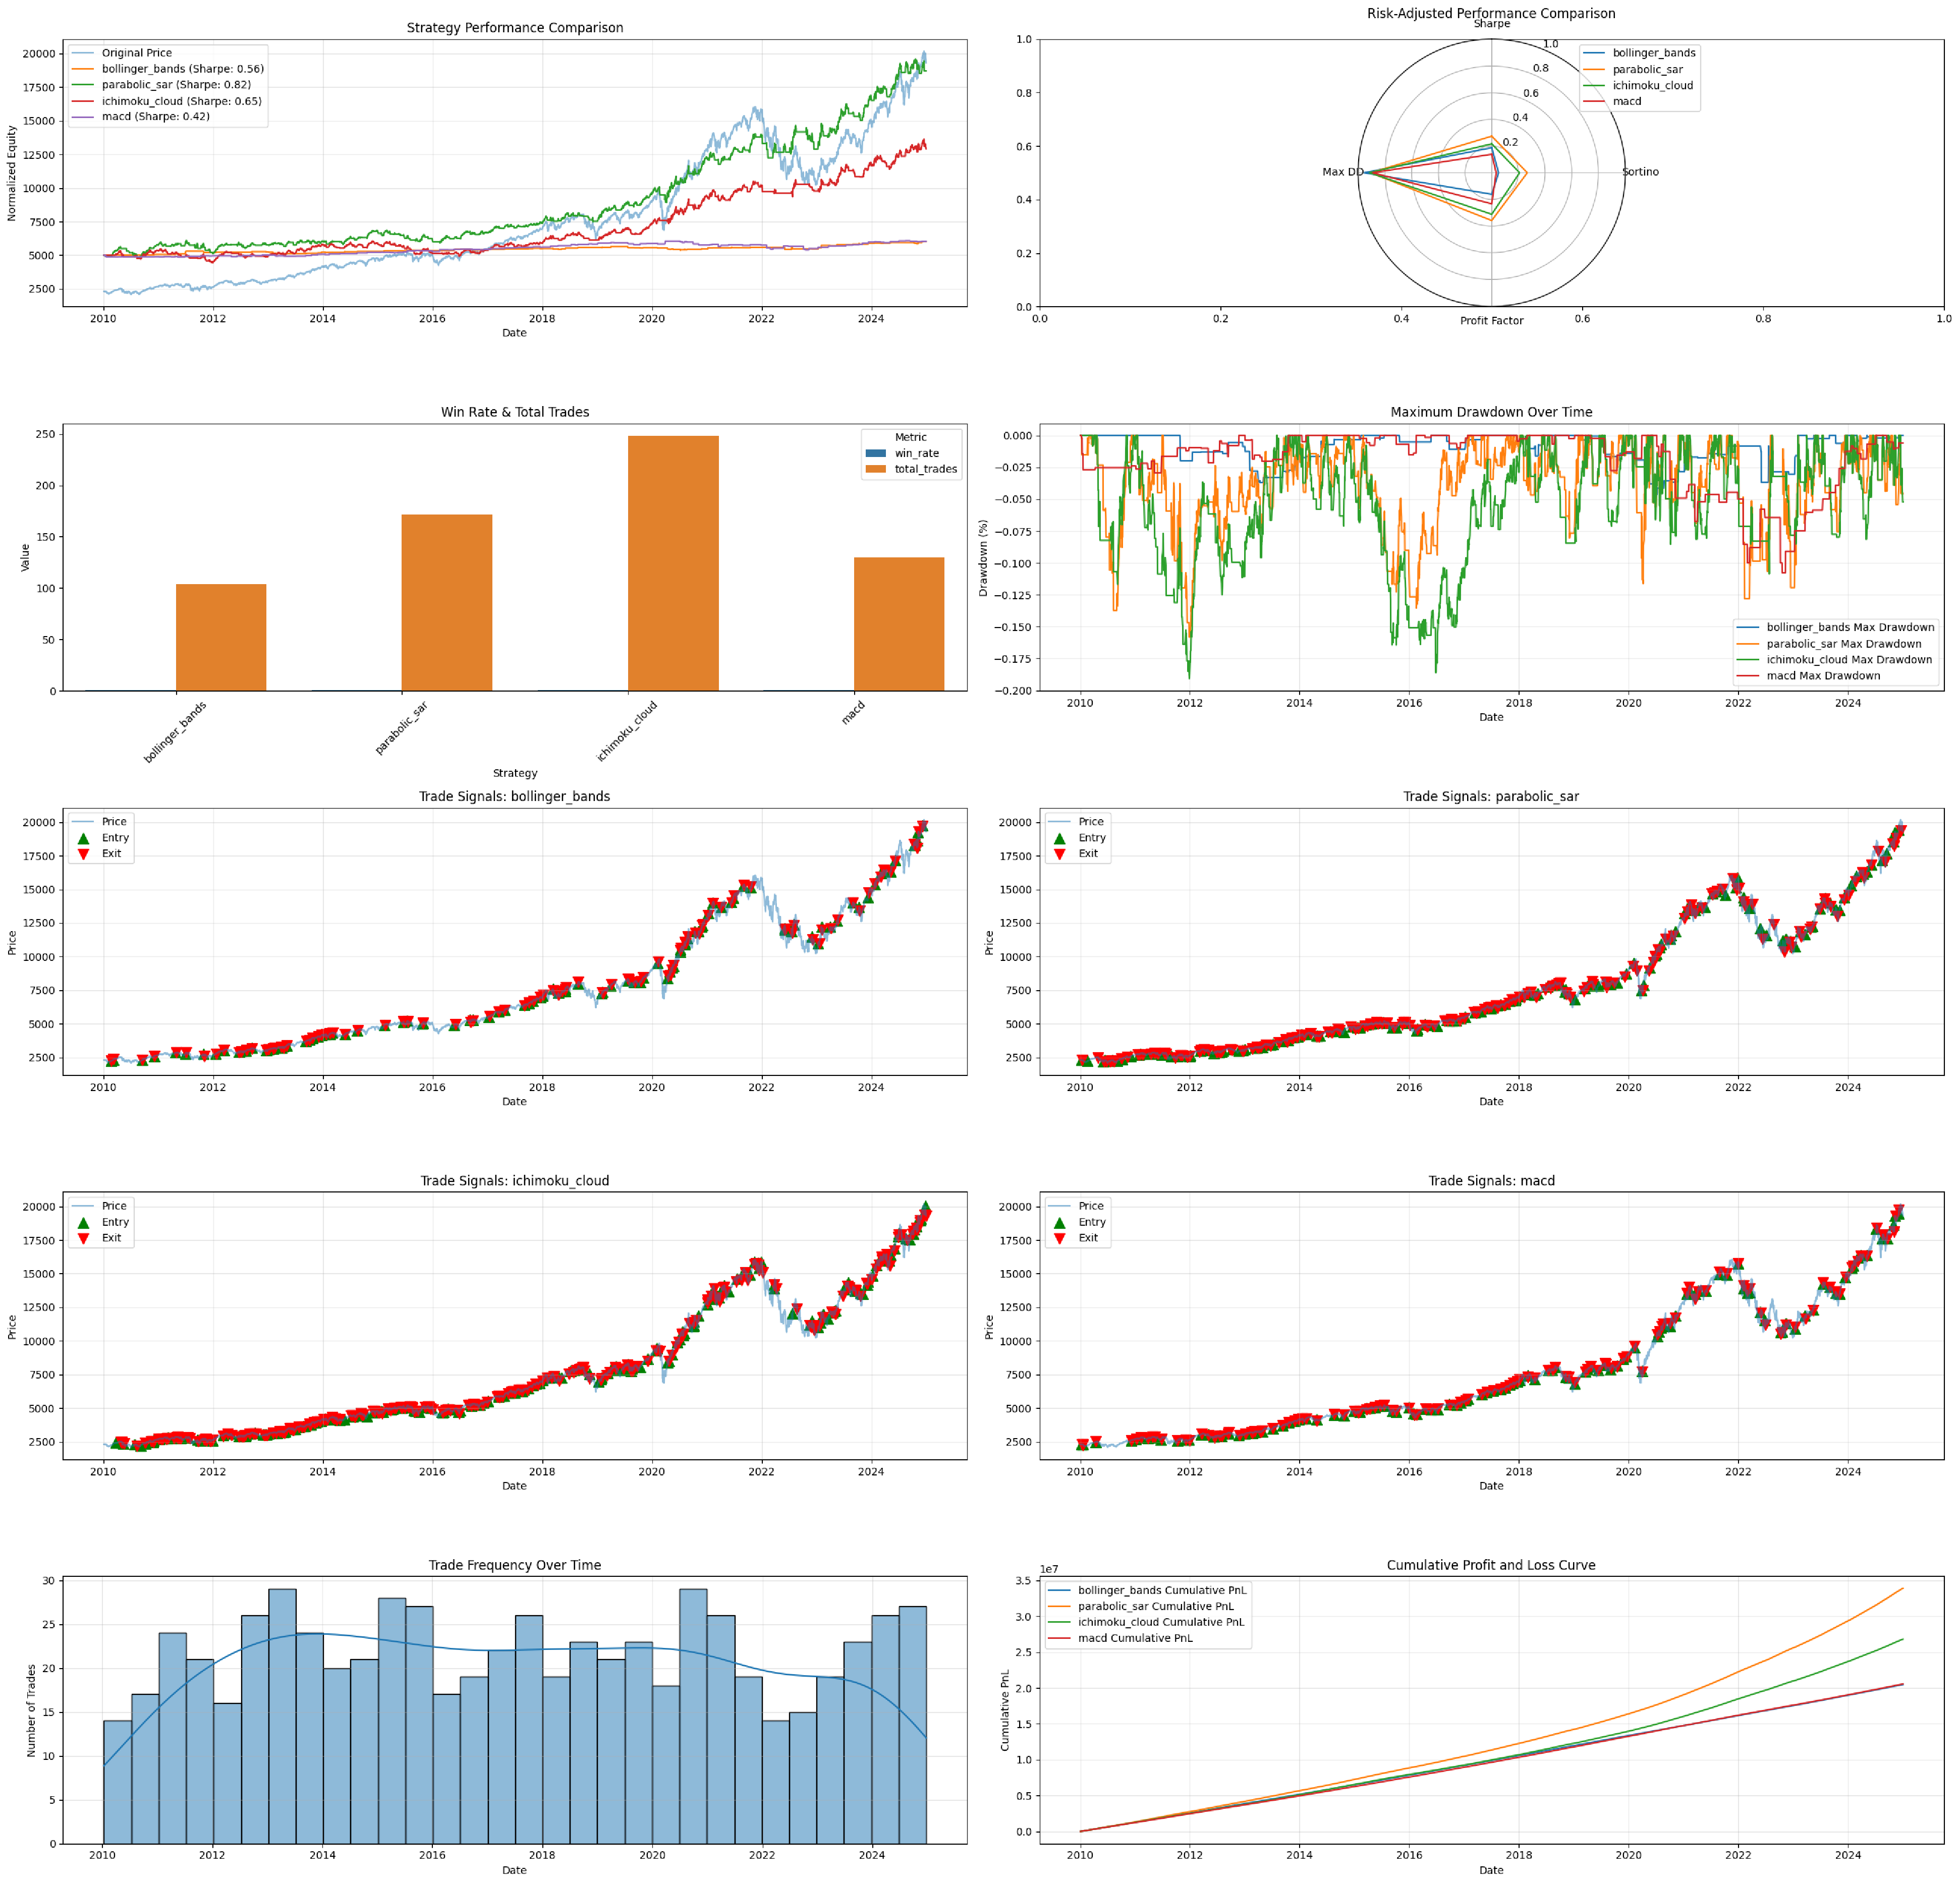
\includegraphics[width=.9\textwidth, height=6.5cm]{bop-out}
        \caption{Bayesian Optimization Workflow}
        \label{fig:bop_architechtar}
    \end{figure}

\subsection{Data Collection, Preprocessing and Strategy Execution}
It all starts with the EnhancedTradingStrategies class, which takes a pandas DataFrame containing Open-High-Low-Close-Volume (OHLCV) data. More than 20 technical indicators (e.g., RSI, MACD, Bollinger Bands, SuperTrend) are used, each one consisting of rules for generating buy and sell signals by combining various precomputed indicators such as RSI, ATR and EMA. For instance, the RSI strategy activates a buy when RSI is below an oversold value (eg 30) and price is above a moving average. An initial balance of 5000 is established and a transaction cost of 0.05\% is included to simulate realistic trading. The run\_strategy method dynamically runs and by emitting buy signals that are then shifted to eliminate look-ahead bias, computing net returns, and plotting equity curves and trades logs (entry/exit dates, prices, returns). The unified execution pipeline provides a uniform execution for all strategies while still providing customization through parameters.

% \begin{equation}
% I_k(t, \theta_k) = F_k(\{X_{t-i}\}_{i=0}^{\tau_k}, I_k(t-1, \theta_k), \theta_k)
% \end{equation}
% \begin{equation}
% F_k =
% \begin{cases}
% R_k(\{X_{t-i}\}_{i=0}^{n_k-1}, \theta_k) & \text{rolling} \\
% E_k(X_t, I_k(t-1, \theta_k), \theta_k) & \text{recursive} \\
% C_k(\{X_{t-i}\}_{i=0}^{t-1}, V_{t-i}, \theta_k) & \text{cumulative}
% \end{cases}
% \end{equation}


\textbf{Parameter Optimization: }
Strategyoptimizer class uses bayesian optimization (BO) from bayes\_opt library to improve performance. For each strategy, define a parameter space (e.g. RSI period: 5–20, MACD fast: 8–20) and BO maximizes the Sharpe ratio by running 20 iterations (5 initial random points + 15 optimized steps). BO (Bayes Optimization) fits a Gaussian Process surrogate that captures the relationship between parameters and Sharpe ratio, that newly selected parameter sets are iteratively selected via an acquisition function (ex: Expected Improvement). Optimized parameters are validated (i.e., periods that are integers) and returned to the strategy execution phase, where the result is refined. By taking automatic steps based on data analysis, rather than manual tuning, this feature aligns well with the project’s research objectives.

\textbf{Indicators Representation}

For \( k = 1, \ldots, 20 \), indicators \( I_k(t, \theta_k) \) from OHLCV data (\( X_t \in \{O_t, H_t, L_t, C_t, V_t\} \)):

\begin{align}
&I_k(t) = F_k(\text{OHLCV}, \theta_k) = 
&\begin{cases}
\frac{1}{n_k} \sum_{i=0}^{n_k-1} f_k(\text{OHLCV}_{t-i}) & \text{if rolling} \\
\alpha_k I_k(t-1) + (1 - \alpha_k) g_k(\text{OHLCV}_t) & \text{if recursive} \\
\sum_{i=0}^{t-1} h_k(\text{OHLCV}_{t-i}, V_{t-i}) & \text{if cumulative}
\end{cases}
\end{align}

\textbf{Optimization}

\begin{align}
&\theta^* = \text{Best}_\theta \left[ SR(\theta) = \frac{\text{profit}}{\text{risk}} \sim \text{GP}(m, k) \right], \\
&\text{where} \notag \\
&SR(\theta) \text{ uses } I_k(t) = F_k(\text{data}, \theta_k), \\
&\theta_k = \{ n_k, m_k, \ldots \}, \\
&m = 0, \quad k(\theta, \theta') = \exp\left(-\sum_{k} (\theta_k - \theta_k')^2\right)
\end{align}
where, linking indicators \( I_k(t) \) with settings \( \theta_k \), scored by \( SR(\theta) \), and optimized via GP and BO


% \begin{itemize}
%     \item \( \theta^* \): Best settings found by BO.
%     \item \( \text{Best}_\theta \): BO’s optimization process.
%     \item \( SR(\theta) = \frac{\text{profit}}{\text{risk}} \): Sharpe ratio from strategy with settings \( \theta \).
%     \item \( \sim \text{GP}(m, k) \): GP predicts \( SR(\theta) \) with:
%     \item \( m = 0 \): Starting guess (mean), assuming no bias initially.
%     \item \( k(\theta, \theta') = \exp\left(-\sum_{k} (\theta_k - \theta_k')^2\right) \): Similarity, where closer settings \( (\theta_k - \theta_k') \) give similar scores.
%     \item \( I_k(t) = F_k(\text{data}, \theta_k) \): Indicators from data, tuned by settings.
%     \item \( \theta_k = \{ n_k, m_k, \ldots \} \): Settings for indicator \( k \).
% \end{itemize}


\subsection{Performance Analysis and Visualization}
The performance is assessed via metrics including Sharpe ratio, Sortino ratio, profit factor, and maximum drawdown computed in calculatemetrics. Three outputs are generated by the StrategyVisualizer class: equity curves for comparing cumulative returns, trade signal plots with entry/exit points on price charts, and bar/radar charts to compare metrics across strategies. Matplotlib and Seaborn are some of the tools used to create visuals that are clearly presented and aligned with the date. The methodology (assuming a user-loaded OHLCV dataset, such as Yahoo Finance) operates in Jupyter or Colab so coupled experimental iterations can be performed.

    \begin{figure}[htbp]
        \centering
        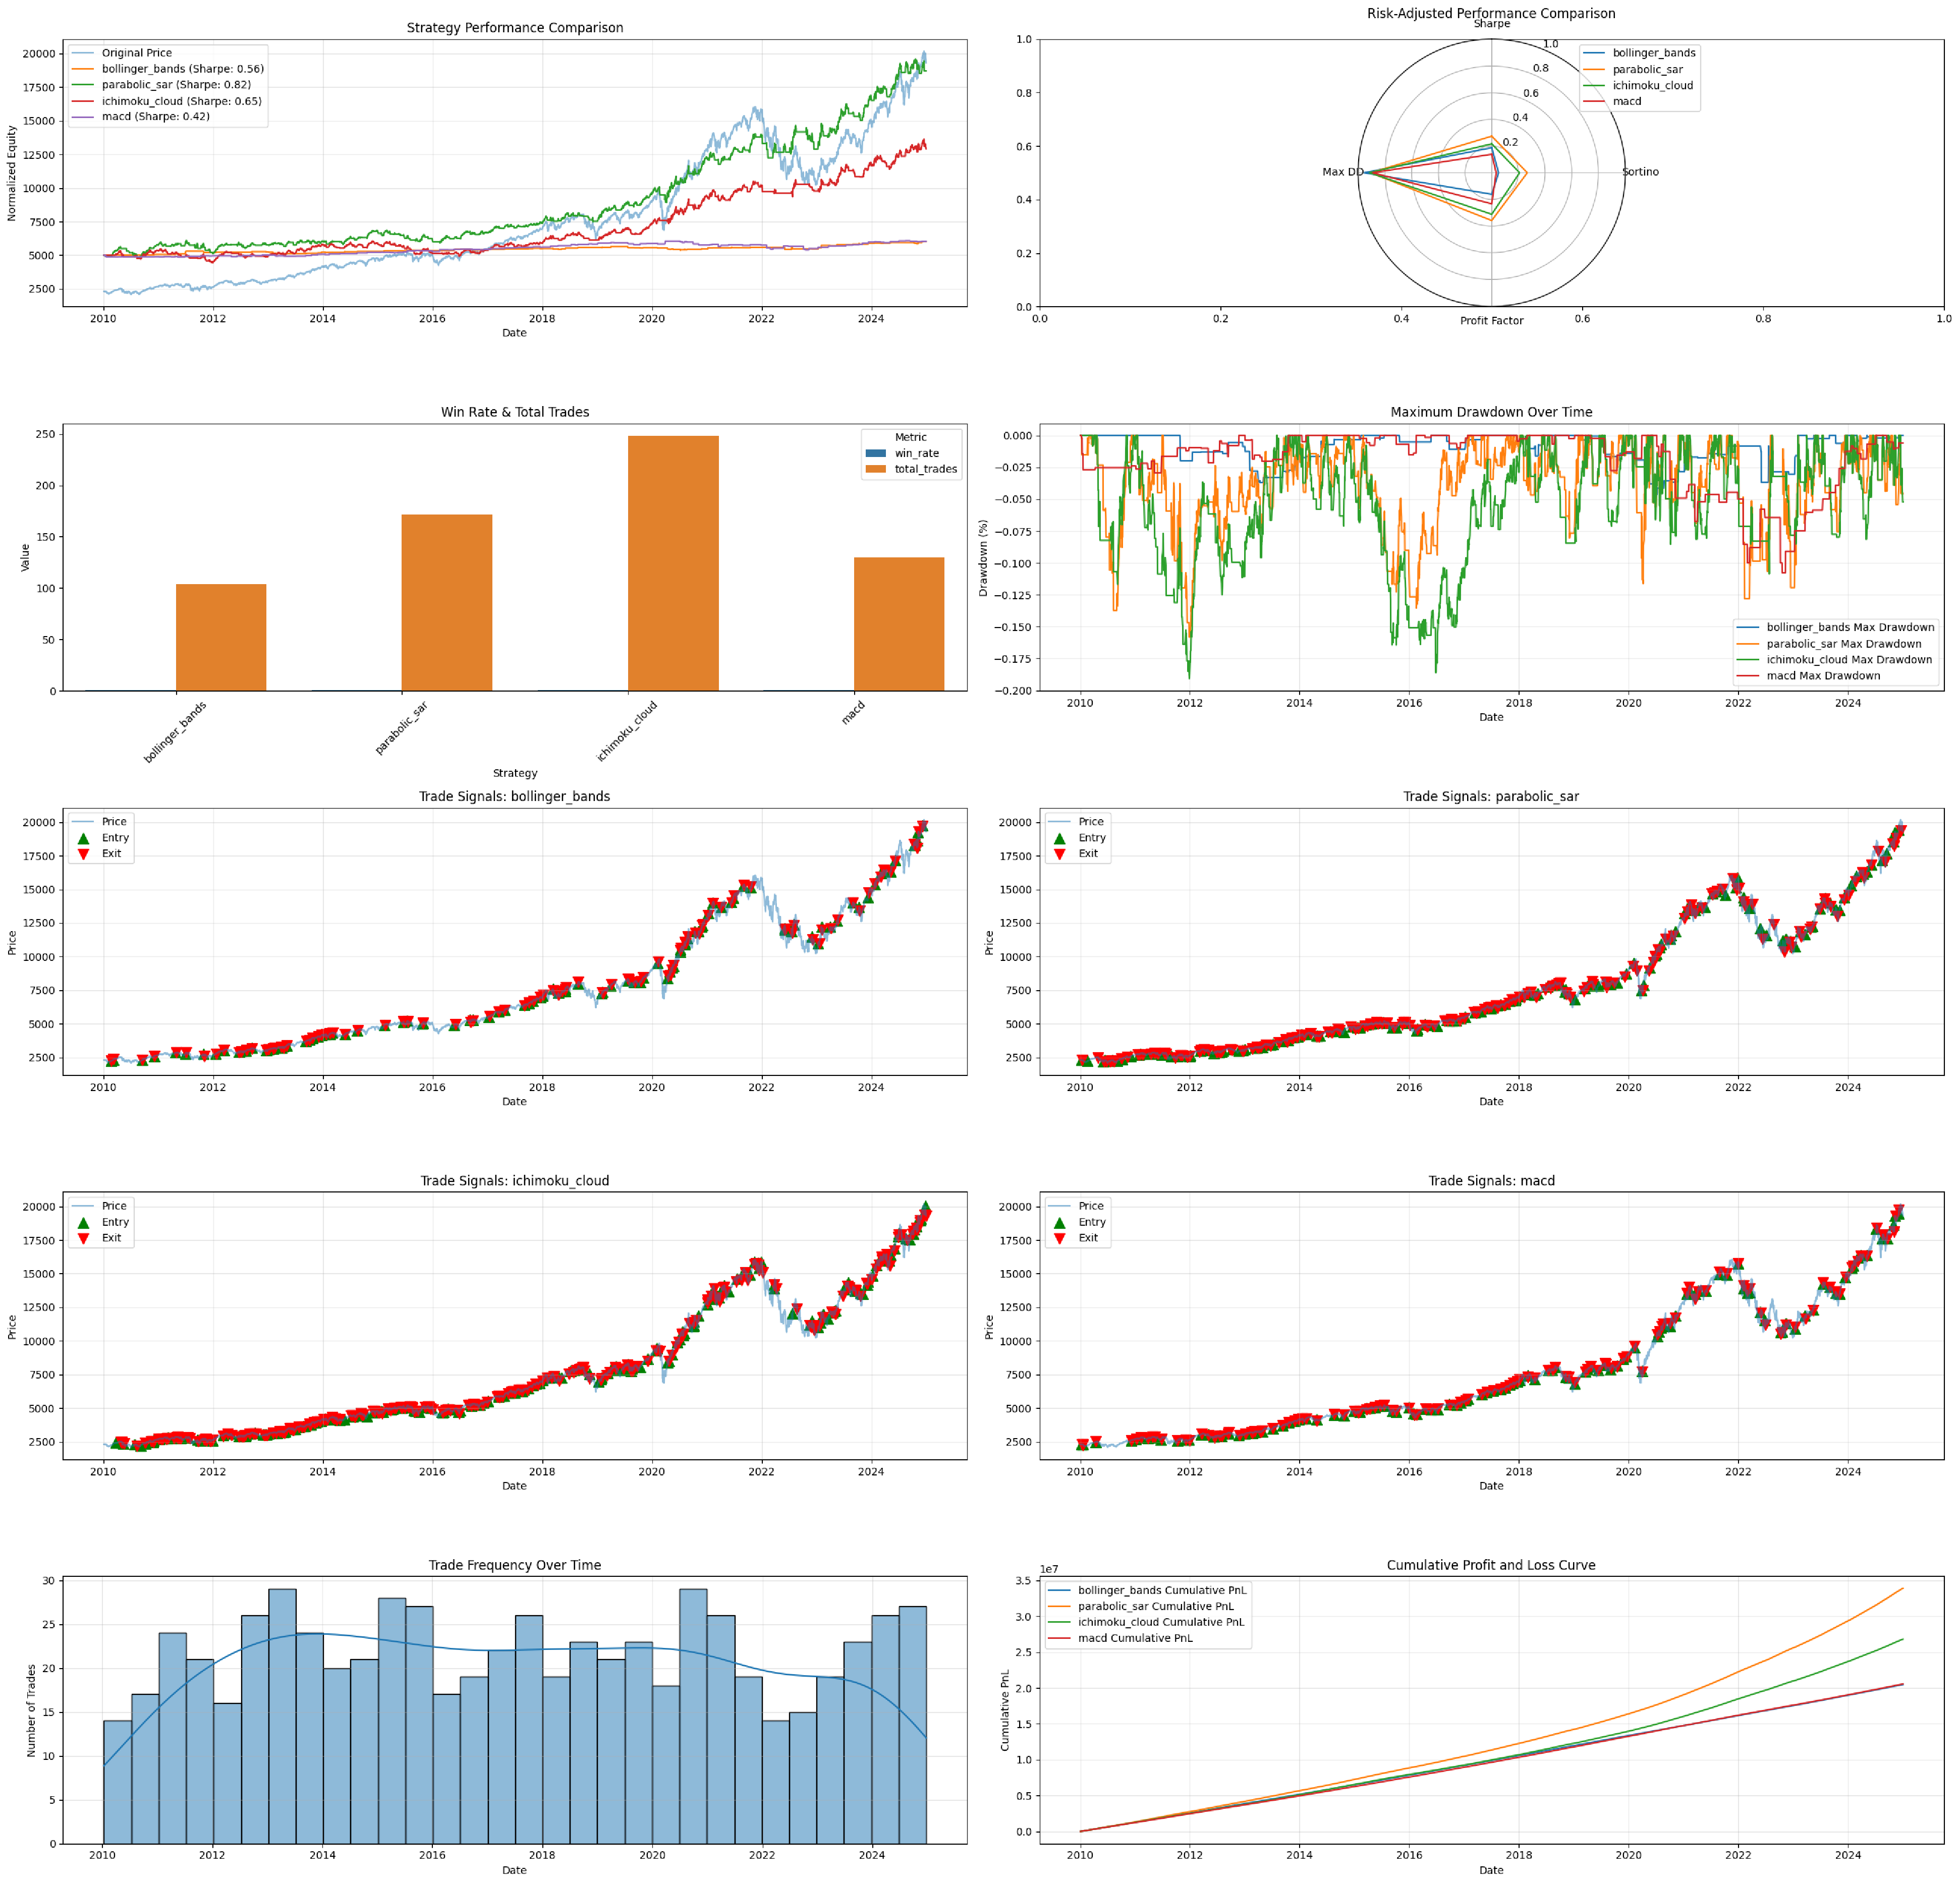
\includegraphics[width=.9\textwidth, height=6.5cm]{bop-out}
        \caption{Bayesian Optimization Performance Analysis}
        \label{fig:bop_performance}
    \end{figure}

This approach also builds a solid framework for the trading research pipeline, by systematically linking strategy design, BO-based optimization, and extensive evaluation.

\section{Algorithm Overview}
The 'StrategyOptimizer' algorithm is a BO-based Sharpe ratio maximizer that tunes trading strategies. 

\begin{table}[h]
\small
\centering
\begin{tabular}{|p{10cm}|}
\hline
\textbf{Algorithm 2 Strategy Optimization with Bayesian Selection} \\
\hline
\textbf{Input:} data (OHLCV DataFrame), $\mathcal{S} = \{ S_1, \ldots, S_m \}$, each $S_i$ with $\theta$ bounds $P[S_i]$, confidence threshold $X$, selected strategies $\mathcal{A} = \{ \}$ \\
\textbf{Output:} results (params, metrics, equity per strategy) \\
\hline
1: \textbf{for each} $S_i \in \mathcal{S}$ \textbf{do} \\
2: \quad Define Obj($\theta$): \\
3: \quad\quad result = RunStrat($S_i$, $\theta$, data); \\
4: \quad\quad \textbf{return} $SR(\theta) = \frac{\text{profit}}{\text{risk}}$; \\
5: \quad Opt = BayesOpt(Obj, $P[S_i]$, init=5, iter=15); \\
6: \quad $\mathcal{A}_i \leftarrow \text{Best}_\theta \left[ SR(\theta) \sim \text{GP}(m=0, k(\theta, \theta')=\exp(-\sum_k (\theta_k - \theta_k')^2)) \right]$; \\
7: \quad \textbf{for each} $\theta \in \mathcal{A}_i$ \textbf{do} \\
8: \quad\quad \textbf{if} $SR(\theta) > X$ \textbf{then} \\
9: \quad\quad\quad $\mathcal{A} \leftarrow \mathcal{A} \cup \{ \theta \}$; \\
10: \quad\quad \textbf{end if} \\
11: \quad \textbf{end for} \\
12: \quad results[$S_i$] = RunStrat($S_i$, $\mathcal{A}_i$[0], data); \\
13: \textbf{end for} \\
14: \textbf{return} results \\
\textbf{Sub:} RunStrat($S_i$, $\theta$, data): \\
15: \quad ts = EnhancedTradingStrategies(data); \\
16: \quad result = ts.$S_i$($\theta$); \\
17: \quad \textbf{return} result['metrics'], result['equity'], result['trades'] \\
\hline
\end{tabular}
\caption{Strategy Optimization with Bayesian Selection}
\label{tab:strategy_optimizer}
\end{table}


It receives OHLCV data and a parameterization of a set of strategies \(\mathcal{S} = \{ S_1, \ldots, S_m \}\), each defined with parameter bounds \(P[S_i]\), and a confidence threshold \(X\). For every strategy \(S_i\) it instantiates the objective function which validates parameters \(\theta\), runs the strategy using 'EnhancedTradingStrategies', and calcs the Sharpe ratio  \(SR(\theta) = \frac{\text{profit}}{\text{risk}}\). BO itself uses a GP with a zero mean and squared exponential kernel to model \(SR(\theta)\), optimizing over 5 initial points and 50 iterations. Giving you. For the top parameters \(\mathcal{A}_i\) and filtering where \(SR(\theta) > X\), we combine them into \(\mathcal{A}\) and the algorithm re-runs each strategy on the best parameters collecting metrics (Sortino, profit factor, etc), equity curves and trades into a dict finaly allowing descriptive insights trading strategy refinement via performance analysis and visualization.

\subsubsection{Result}
The trading strategy performance analysis is based on tweenty strategies and here are the top nine, including parabolic\_sar, ichimoku\_cloud, macd, etc.The evaluation period was carried out over 2023 and 2024. The Sharpe ratio, an important performance evaluation number, varies from -0.494 (keltner\_channel) to 1.665 (macd), pointing that macd is the most efficiently risk adjusted profitable strategy, while keltner\_channel underperforms with negative returns. The macd and parabolic\_sar types stand out (1.942, 2.750) with sortino ratios and profit factors indicating low max drawdowns (e.g. 0.011 for macd) and robust risk management. Total trades range from 16 to 93, and obv\_strategy delivers a high number of trades with moderate profitability. 

SO where do you think this Genesis of Coin show us after 1,891 days on the scroll. Final balances where available max out at 7467.281 (parabolic\_sar) reflecting strong cumulative returns. The totals with balance and without balance repeat most of the times, this means that there have been multiple runs of the evaluation, which may indicate that the different metrics were stable, but the final balances were different.

\begin{table}[h]
\tiny
\centering
\begin{tabular}{|c|c|c|c|c|c|c|c|c|c|}
\hline
\textbf{Strategy} & \textbf{Sharpe} & \textbf{Sortino} & \textbf{Profit Factor} & \textbf{Max Drawdown} & \textbf{Total Trades} & \textbf{Score} & \textbf{Final Balance} \\
\hline
parabolic\_sar & 1.633 & 1.942 & 2.750 & 0.061 & 22 & 1.633 & 7467.281 \\
ichimoku\_cloud & 1.105 & 1.163 & 1.933 & 0.074 & 34 & 1.105 & 6323.770 \\
macd & 1.665 & 1.473 & 1.772 & 0.011 & 21 & 1.665 & 5490.222 \\
vwma\_crossover & 1.515 & 1.635 & 2.639 & 0.073 & 16 & 1.515 & 7138.089 \\
keltner\_channel & -0.494 & -0.292 & 1.110 & 0.138 & 39 & -0.494 & 4642.744 \\
fibonacci\_retracement & 1.398 & 0.634 & 0.586 & 0.027 & 30 & 1.398 & 5497.101 \\
williams\_r & 1.373 & 0.737 & 1.901 & 0.024 & 19 & 1.373 & 5693.641 \\
cmf & 1.307 & 1.419 & 2.111 & 0.073 & 21 & 1.307 & 6758.628 \\
obv\_strategy & 1.650 & 1.702 & 1.231 & 0.079 & 93 & 1.650 & 6944.823 \\
\hline
\end{tabular}
\caption{Performance Metrics of Trading Strategies with Final Balance}
\label{tab:ob_strategy_performance}
\end{table}

\section{Conclusion}
As such, MACD and parabolic\_sar are the winners compared to the other strategies with Sharpe ratios (1.665, 1.633 respectively) and good profit factors as well, as well as comparatively low drawdowns, which enable them for trading being risk-adjusted. Negative Sharpe ratio (-0.494) of Keltner\_channel indicates its poor performance requiring parameter tuning. obv\_strategy with 93 trades showed moderate profit with a high trading frequency, improving refinement probably possible. Such variation in the report of final balances across the entries suggests that standardized evaluation may be necessary. Provide an overview of what you are doing is important and how to choose hybrid strategies combining macd and parabolic\_sar for consistent metric reporting maximizing profitability with low risk exposure in a dynamic market conditions.